\documentclass[../main.tex]{subfiles}
% !TEX root= ../main.tex

\begin{document}
\subsection{Overhead}
Overhead is the work the parallel code has to do that isn't needed in the sequential program.

\begin{itemize}
	\item \textbf{Communication:} parallel processes need to exchange data.
	      Example: Reduce
	      \begin{center}
		      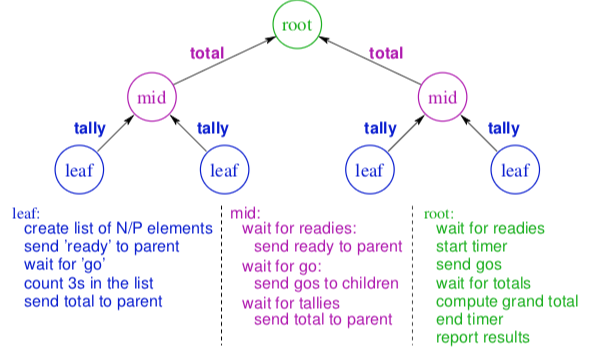
\includegraphics[scale=0.65]{images/scan-communication.png}
	      \end{center}

	      \begin{itemize}
		      \item \texttt{shared memory:} The caches communicate to make sure that all references from different cores to the same address look like there is one, common memory. Global memory access overhead is longer than shared memory access.
		      \item \texttt{message passing:} The time to transmit the message through the network. The time set up the transmission and the time to receive the message, etc.
		      \item {
		            \texttt{GPU Example:}
		            \begin{itemize}
			            \item GPUs communicate using memory, and memory accesses are slow. Threads in the same block can communicate using shared memory, which is fairly fast. Communication between different requires using global memory -- either by using atomics or by launching multiple kernels. These global memory accesses introduce communication overhead that can be very large.
			            \item Communication between CPU and GPU involves slow, global-memory access.
		            \end{itemize}
		            }
	      \end{itemize}
	\item \textbf{Synchronization:} Parallel processes may need to synchronize to guarantee that some operations (e.g. file writes; access to shared data structures) are performed in a particular order. For a sequential program, this ordering is provided by the program itself.
	      \begin{itemize}
		      \item \texttt{shared memory:} there are explicit locks or other synchronization mechanisms.
		      \item \texttt{message passing:} synchronization is accomplished by communication.
		      \item {
		            \texttt{GPU Example:}
		            \begin{itemize}
			            \item Calls to \code{\_\_syncthreads()} incur synchronization overhead.
			            \item Using multiple kernels to provide communication between blocks. All threads in one kernel must complete execution before the next kernel is launched.
		            \end{itemize}
		            }
	      \end{itemize}
	\item \textbf{Computation Overhead:} A parallel program may perform computation that is not done by the sequential program, e.g. redundant computation: it is faster to recompute the same thing on each processor than to broadcast.
	      \begin{itemize}
		      \item \texttt{GPU example:} anytime a value is recomputed by multiple threads.
	      \end{itemize}
	\item \textbf{Memory Overhead:} Each process may have its own copy of a data structure.
\end{itemize}

\subsection{Limited Parallelism}

\begin{itemize}
	\item \textbf{Non-parallelizable code:} something that has to be done sequentially.
	\item \textbf{Idle Processors:} There's work to do, but some processor are waiting for something before they can work on it.
	      \begin{itemize}
		      \item Start-up and completion cost.
		      \item Work imbalance.
		      \item Communication delays.
		      \item {
		            \texttt{GPU example:}
		            \begin{itemize}
			            \item Thread divergence, e.g, when only some SPs are active during a reduce.
			            \item If a SM doesn't have enough warps, then the SM will be idle on cycles that the warp-schedule cannot issue an instruction.
		            \end{itemize}
		            }
	      \end{itemize}
	\item \textbf{Resource Contention:}
	      \begin{itemize}
		      \item Too many processors overloading a limited resource.
		      \item It's easy to change a compute-bound task into an I/O bound one by using parallel programming.
		      \item Network bandwidth.
		      \item \texttt{GPU example:} Bank conflicts when accessing shared memory.
	      \end{itemize}
\end{itemize}

\end{document}
